
%%% N.B. please use English grammar consistently, all Americanisms should be avoided. Therfore Polarisation, not Polarization is the correct way of writing. The Practicum guide is awfully inconsistent. 
% Also Set-up is always (both in Engish and American) written with hyphen
%%%

\documentclass[11pt,a4paper]{article}
\usepackage[english]{babel}
\usepackage{graphicx}
\usepackage{subcaption}
\usepackage{epstopdf}
\usepackage{amsmath}
\usepackage{amssymb}
\usepackage{fixltx2e}
\usepackage{float}
%\usepackage[numbered]{mcode}
\usepackage{listings}
\usepackage[margin=1in]{geometry}

\newcommand{\mat}[1]{\begin{bmatrix}#1\end{bmatrix}}

\begin{document}

\noindent
\begin{center}
\includegraphics[width=\columnwidth]{tudelftlogo.eps} \\

EE3P11 Electromagnetics\\
\begin{LARGE}
\textbf{Practicum Session 2 \\ Free Space Propagation of EM Waves} \\[0.3cm]
\end{LARGE}
\today \\[.2cm]
\begin{tabular}{l l}
Dani\"el Booms & 4284216 \\
Piet De Vaere & 4304241 \\
Nicolaas du Plessis & 4203933 \\
Job van Staveren & 4317386

\end{tabular}
\end{center}


\subsection*{Introduction}
The second session of the practicum for EE3P11 Electromagnetics consists of two parts.
In the first part about free space propagation, some experiments are done about propagation velocity, signal power, absorption and the influence of polarisation.
The second part of this session is about the polarisation state of EM waves with and without multi-path propagation.
Using the polarisation pattern method, the polarisation state of the EM waves will be determined.


\section{Free Space propagation}

The first experimental set-up was used to investigate free space propagation of electromagnetic waves between two antennae.
The set-up consisted of a transmitter and a receiver antenna separated in free space, as can be seen in the experimental set-up in figure \ref{fig:setup_one}.
The transmitter used a klystron-based microwave generator to modulate a reference signal with the RF signal, which had a fixed frequency of $9.475$ GHz.
With the horn orientation of the transmitter antenna shown in the set-up, the transmitted electric field component was travelling horizontally through space, i.e. in and out of the page.\\

\begin{figure}[H]
\begin{center}
\includegraphics[scale=0.5]{setup_one.PNG}
\caption{Measurement Set-up Experiment 1 [2]}
\label{fig:setup_one}
\end{center}
\end{figure}

The receiver had a freely rotatable horn antenna, and used a heterodyne detector to mix the received wave with a reference wave in order to down shift the frequency to a more measurable level. This non-linear process also involves a quadratic term, which results in the output amplitude (voltage) being proportional to the received wave's power. The output was therefore  attached to a speaker, where the volume was proportional to the received amplitude of the EM carrier wave and the amplitude of the modulated reference signal. This meant that any change in the transmitted power would be heard as a change in volume in the speaker, and would appear as a change in voltage on the voltmeter.\\

Normally, the measured voltage of an EM wave is the induced voltage by the electro-motive force, which when measured with a voltmeter only gives information about the amplitude of the wave. As we are looking at propagation of an EM wave, we are interested in the power of the wave. As any information is normally frequency modulated onto an EM wave, the amplitude does not carry information. Therefore information, or signal strength, would only be dependent on the power. This is why it is important to show that the heterodyne detector output of the experimental setup squares the amplitude internally, meaning that the actual voltage of the output is proportional to the wave's power, and can be used to quantitative examine the propagation quality. All subsequent voltages shown in the experimental data can be seen as power and be compared as such, albeit with an unknown scale factor.

\subsection{Wavelength and propagation in free space}
In order to measure the wavelength of the EM wave packets, we would have to fix the EM wave in position through space. This is done by placing a metal grid with the wires in the vertically orientation in between the transmitter and receiver. This grid forces the electric field to be zero at that point, meaning that a standing wave at the EM wave frequency forms between the antennae and the grid.\\

By moving the grid along the path between the antennae, when the volume of the radio is at a minimum, the grid is located at a minimum anti-node of the wave package. Therefore, by measuring this phenomenon at different locations, we can estimate the wavelength of the standing wave. The measured minimum amplitude locations were found at the positions as shown below in table \ref{tab:1.1_results}. The transmitter horn was located at the 60cm mark, and the receiver at the 120cm mark.\\

\begin{table}[H]
\centering
\caption{Standing Wave Local Minimum Locations.}
\label{tab:1.1_results}
\begin{tabular}{| l | l |}
  \hline
  \textbf{Measured Voltage [V]} & \textbf{Position [cm]} \\ \hline
  0.35 & 92.1 \\ \hline
  0.38 & 90.3 \\ \hline
  0.40 & 88.5 \\ \hline
\end{tabular}
\end{table}

From the data above, the separation of anti-nodes is 1.8cm, which means that the wavelength of the standing wave is $2 \cdot 1.8 = 3.6cm$. The phase velocity of the standing wave is therefore $v = f \times \lambda = 9.1 \cdot 10^9 \times 36 \cdot 10^{-3} = 3.28 \cdot 10^8$ m/s. As found in the last lab session, the phase velocity here is above the speed of light in a vacuum, which is counter intuitive. Taken from the previous session's explanation [3]:
\begin{quotation}
While the phase velocity represents the velocity of a single frequency component of the wave, it does not take into account the individual propagation delays of each component between the two points. [...] Due to these separated occurrence, no information can be transmitted at such speeds, making the phase velocity an essentially useless observation that gives no usable information on the compound waveform.''
\end{quotation}

\subsection{Relation between the received signal and propagation distance}
The power transmitted between the transmitting and receiving antenna is dependent on the propagation distance, i.e. the distance between the antennae. Assuming that:
\begin{equation}
Signal Voltage \propto \frac{1}{distance^{x}}
\end{equation}, 
we can estimated x based on measured data given in table \ref{tab:1.2_results}.

\begin{table}[H]
\centering
\caption{Antenna Separation and Signal Strength}
\label{tab:1.2_results}
\begin{tabular}{| l | l |}
  \hline
\textbf{Antenna Separation [cm]} & \textbf{Measured Voltage [V]}\\ \hline
40  & 4.14 \\ \hline
50  & 3.46 \\ \hline
60  & 2.86 \\ \hline
70  & 2.27 \\ \hline
80  & 1.74 \\ \hline
90  & 1.33 \\ \hline
100 & 1.07 \\ \hline
110 & 0.86 \\ \hline
120 & 0.75 \\ \hline
130 & 0.63 \\ \hline
140 & 0.52 \\ \hline
150 & 0.45 \\ \hline
160 & 0.39 \\ \hline
170 & 0.36 \\ \hline
\end{tabular}
\end{table}

By plotting the data and using a curve fitting tool, the closest fit in the form of:
\begin{equation}
Voltage = a \times \frac{1}{distance^r}
\end{equation}
 is when $a = 1106 \: V^{-1}cm^{-2}$, and $r = 1.492$, with a confidence value of $R^2 =  0.97$. Here we see that $a$ is a scalar constant, and $r$ shows the relationship to be to the power of 1.5. In reality, we know the inverse-square law results in the power decreasing at the distance squared, so we would expect the result to be $r=2$. While this result does not fall within the statistical confidence interval, the value is close enough, as the large uncertainties in the experiment are difficult to quantify, and therefore cannot readily be taken into account. \\

\begin{figure}[H]
\begin{center}
\includegraphics[width=\textwidth]{curve_fit_1_2.png}
\caption{Fitted Data from Table \ref{tab:1.2_results}}
\label{fig:fit_1.2}
\end{center}
\end{figure}

\subsection{Transmission and absorption of EM waves on flat objects}\label{sec:objectsInPath}
In an investigation into the effects of different objects on the propagation of the EM wave, these objects were placed between the two antennae, and the resulting voltages measured on the volt meter were recorded. The antennae were both orientated in the vertical polarisation, and with a separation of 120cm. The objects were all place 90cm from the transmitting antenna, and the resulting voltage was recorded below in table \ref{tab:1_3resutls}. \\

\begin{table}[H]
\centering
\caption{Objects with results voltage}
\label{tab:1_3resutls}
\begin{tabular}{| l | c |}
  \hline
\textbf{Object} & \textbf{Measured Voltage [V]}\\ \hline
Free Space  & 2.040 \\ \hline
Metal Plate & 0.075 \\ \hline
Dielectric Plate  & 1.970 \\ \hline
Absorbing Material  & 0.030 \\ \hline
Wire Grid (Vertical)  & 0.060 \\ \hline
Wire Grid (Horizontal)  & 1.900 \\ \hline
\end{tabular}
\end{table}

As mentioned at the beginning of the section, the displayed voltage is equivalent to the power of the transmitted EM wave. We can therefore draw the following conclusions about the above mentioned materials.\\

\begin{itemize}
\item In free space, the EM wave travels without hindrance, where the only significant losses those associated with dissipation over distance.
\item The metal plate forces the electric field component to be zero at all points in the plane, and the magnetic component loses it's energy by inducing eddy currents in the plate. A standing wave is created, but is heavily damped due to the energy losses in the metal plate.
\item The dielectric material acts as an insulator, so energy is not dissipated by induced eddy currents. The electric field is also not bound, as the polarization in the material allows the dielectric to follow the electric field at that point. 
\item The absorbing material does what the name implies. Similar to the metal plate, but dampens reflections from the incident wave, further preventing the signal from propagation around the object through external reflections.
\item With the gird wires perpendicular to the electric component's oscillation, the EM wave is dampened. This is due to the electric field being fixed throughout the object, and the magnetic field inducing a current in the object that can flow in a loop. This current loop (eddy current) heats up the material due to the resistance of the metal, which is where the dissipated energy goes to.
\item With the grid wires parallel to the electric component, the electric field can pass through the spaces between the wires without being bound to a standing wave, and the magnetic field cannot induce currents (or an electro-motive force) along the length of the wires. The overall results means that little energy is lost.
\end{itemize}

\subsection{The influence of polarisation}
Lastly, the effect of anisotropic structure on the polarisation of the wave was investigated. Firstly, the polarisation isolation is measured between the antennae when they are orthogonally polarised. At an antenna separation of 120cm, the matched orientation of the antennae result in a voltage of $2.14V$, while an orthogonal orientation results in a measured voltage of $0.014V$. Given that 
\[Q = \frac{\text{Signal voltage for orthogonal polarisations of antennas}}{\text{Signal voltage for matched polarisations of antennas}}\] we find that $Q = \frac{0.014}{2.14} = 0.00654 = -21.8 dB$, as the signal voltage is indicative of transfered power.\\

We then considered the antennae orthogonally polarized, and placed the wire grid in between the antennae to see what would happen with the transmitted power. With the grid orientated vertically or horizontally (same polarisation as either antennae), we found that signal voltage to be $14mV$, which shows no difference to when the grid is not present. However, when the grid was rotated 45 degrees, to where the orientation is equally angularly separated from either antennae, we found that the signal level increased to $1V$. \\

This increase is quite significant, as it shows a $18dB$ increase in transmitted energy. While this is not as high as the reference $2.04V$ when the antennae are rotationally aligned, is still shows that a significant amount of energy is propagation from the transmitter to the receiver. This is due to the fact that the re-radiation of the EM wave is maximally at a 45 degree angle.\\

As the metal grid absorbed the energy, the induced eddy currents transmit their own EM wave, the strength of which being dependent on the resistance of the grid, the power of the incident wave, and the angle between the grid and the incident wave's electric field component. The grid re-radiates the EM wave in the same polarisation as the grid's wires, which means that at a 45 degree angle, the wave from the transmitter is effectively absorbed, and re-radiated with a bit of dampening. The re-radiated wave then falls on the receiver, which also undergoes dampening due to the angle difference. The overall results if that the grid allows the EM wave to propagate through space, when it normally be rejected by the orthogonal polarisation of the antennae.

\subsection{Conclusion}
Using the set-up depicted in figure \ref{fig:setup_one}, four experiments were performed.
The first experiment investigated the wavelength and free space phase velocity of a 9.475 GHz EM-wave were determined.
The wavelength was calculated to be 3.6 cm, and the phase velocity $v = 3.18 \cdot 10^8$ m/s.
The phase velocity is higher than the speed of light, which is possible because it is an \emph{apparent} velocity.\\

In the second experiment the attenuation factor of an EM-wave in free space was measured.
The results show that the power of an EM-wave is inversely proportional to the distance to a power of 1.5.
Given the crudity of the experimental set-up, this value is considered to be reasonably close to the expected power of 2.\\

The third experiment investigated the effects of different objects in the propagation path.
The results for different kind of materials are itemized in section \ref{sec:objectsInPath}.\\

The final experiment looked at the influence of polarization.
It was found that the received power is a strong function of the polarisation differences between the receiving and transmitting antennae.
It was also found that by placing a grid of parallel wires in the path of the wave, the polarisation of the wave could be changed due to re-radiation on the EM wave, thus 
altering the received signal power. 


\section{Polarisation state measurements using polarisation pattern method}

\subsection{Measurement Set-up}
The experimental set-up that will be used is shown in figure \ref{fig:exp_setup}. The transmitting antenna is a circular horn antenna. By adjusting the settings of the transmitter, either a vertically polarised or a circularly polarized wave can be transmitted. This wave has a frequency of 9.1 GHz. The receiver antenna is a horn antenna with a linear polarised sensitivity. To measure the polarisation pattern of the transmitted wave, the receiver antenna will be rotated slowly so that it makes a rotation of 360 degrees. During this full rotation the amplitude of the received wave is measured. This makes it possible to measure the entire polarisation pattern as a function of the rotation angle. In the first experiments the metal or dielectric plate, as indicated in figure \ref{fig:exp_setup}, will not be used. Only the absorber is used to eliminate reflections. The final three measurements will be done using either the metal or dielectric plate. The distance $R_0$ = 1.875 m, and the absorber is placed halfway between the two antennae at $R_0/2$ = 0.94 m.

\begin{figure}[H]
\begin{center}
\includegraphics[scale=0.5]{exp_setup.png}
\caption{Measurement Set-up}
\label{fig:exp_setup}
\end{center}
\end{figure}

\section{Theory and calculations}
In [2] it is given that the amplitude of the received wave in case of a linearly polarised transmitted wave can be written as:
\begin{equation}
E_{0r}=A|1+\Gamma e^{jk\Delta R}| = A|1+\Gamma e^{-j2kh_1 h_2/d}| \mathrm{V\cdot m^{-1}}
\label{amplitude}
\end{equation}
Where $h_1, h_2$ are the distances between the transmitter/receiver and the reflecting surfaces. d is the distance between the receiver and transmitter and k is the wave number.\\
Since the receiver and transmitter are at a height of 90.5cm and the metal plate when present is at 77cm, $h_1=h_2=90.5-77=0.135m$. d was found to be 1,875m. For k we have $k=\frac{2\pi}{\lambda}=\frac{2\pi f}{c}=0.199m^{-1}$\\
The only unknown is now the reflection coefficient $\Gamma$. However, since the metal plate is a conductor, we can estimate it by $\Gamma = -1$ for horizontal polarisation and $\Gamma = 1$ for vertical polarisation, this results from applying the boundary conditions for the E-field. When the metal plate is not present, the absorber  is assumed to have a reflection coefficient of $\Gamma = 0$ for both horizontal and vertical polarisation. For the dielectric material $0<\Gamma<1$ and dependent on the angle of incidence, the direction of polarisation, and the permittivity of the dielectric.\\
Figure \ref{fig:e_zero} shows the amplitude according to (\ref{amplitude}) for the distance between reflector and receiver. This figure is normalized to $E_0$ in the case when there are no reflections. Hence the normalized amplitude is bounded between 0 and 2.\\
For circular polarisation it can be derived from [2] that the received polarisation vector can be written as:
\begin{equation}
\overrightarrow{E_{0r}}=A
\begin{pmatrix} 1+\Gamma_{H}e^{jk\Delta R}\\ 1+\Gamma_{V}e^{jk\Delta R} \end{pmatrix} \mathrm{V\cdot m^{-1}}
\label{eq:amplitudeCircular}
\end{equation}
Where $H$ is the same amplitude scalar as in equation \ref{amplitude}, $\Gamma_{H}=-1$ and $\Gamma_{V}=1$ in case of the metal plate. This will result in constructive interference from the reflected wave in some directions, and destructive in directions perpendicular to this. The exact angle of maximal constructive interference depends on $\Delta R$. In case of the dielectric the interference is constructive for all directions but for some more than others, the polarisation will appear more eccentric than without reflection.

\subsection{Results and Conclusion}
Figure \ref{fig:pol_pat} shows the results for the vertical and circular polarised transmitted wave. In this experiment, no metal or dielectric plate is used, only the absorbing material to eliminate the reflections. The received wave therefore shows the polarisation pattern of the transmitted wave. 

%For question 2.1 and 2.2
\begin{figure}[H]
\begin{subfigure}{0.5\textwidth}
  \centering
  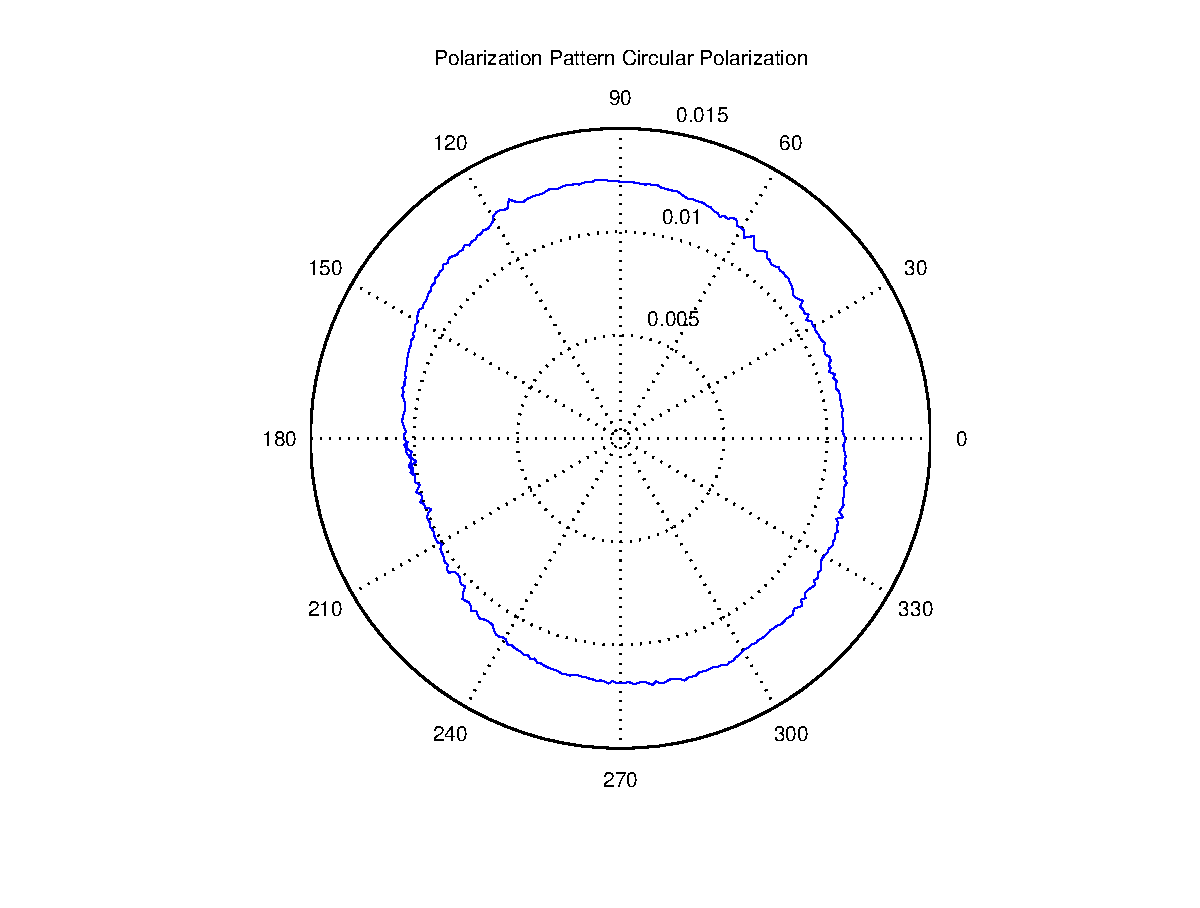
\includegraphics[width=1.2\linewidth]{2_1circ_pol.eps}
  \caption{Circular Polarisation}
  \label{fig:2_1circ}
\end{subfigure}%
\begin{subfigure}{0.5\textwidth}
  \centering
  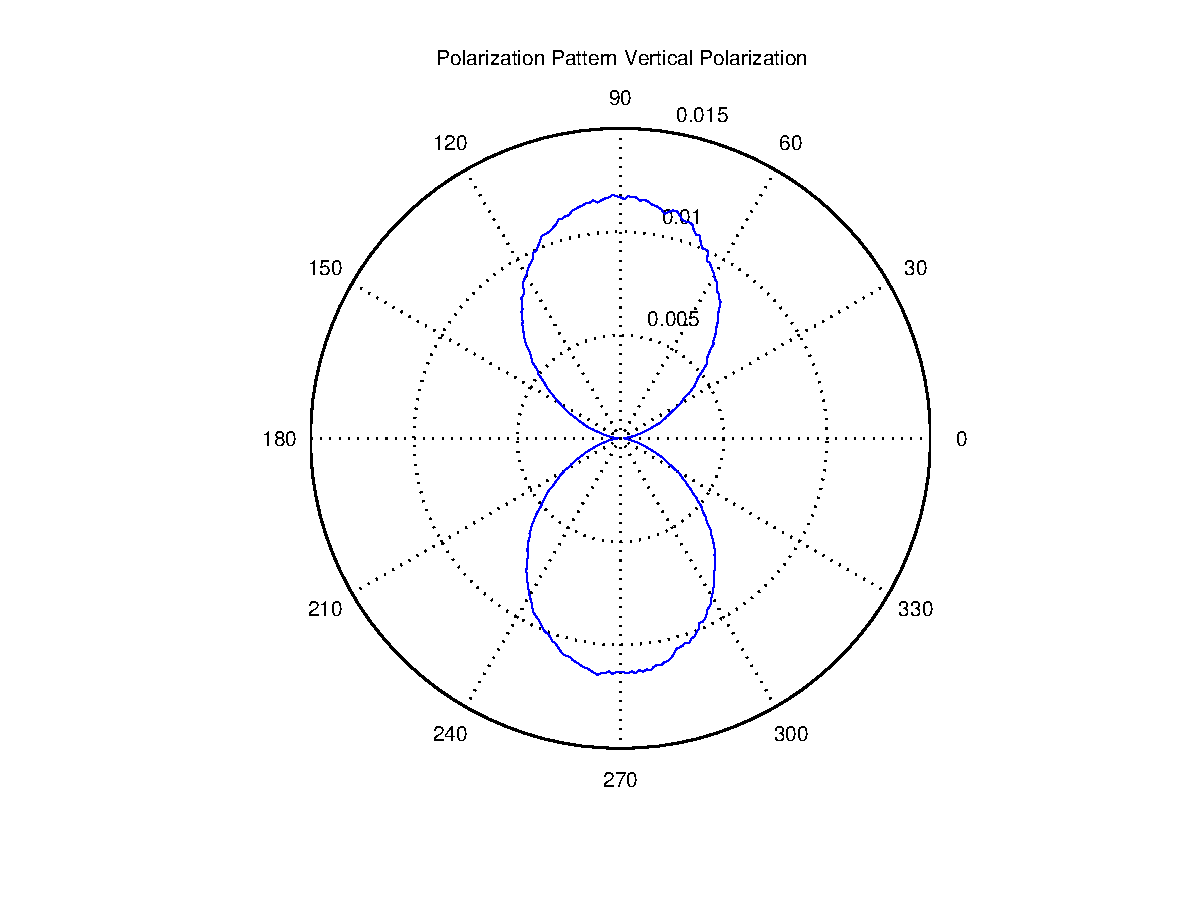
\includegraphics[width=1.2\linewidth]{2_2vert_pol.eps}
  \caption{Vertical Polarisation}
  \label{fig:2_1vert}
\end{subfigure}
\caption{Measured polarisation pattern}
\label{fig:pol_pat}
\end{figure}

For the next two experiments, the metal plate is placed on top of the absorber. The metal plate now introduces reflections. The measurement results are shown in figure \ref{fig:pol_pat_metal_plate}. It can be seen that for the circularly polarised transmitted wave the received wave appears to be almost linearly polarised. The this is the result of the interference of the reflected wave. The maximum amplitude of the received field, located around 160 an 340 degrees, is larger than without a reflected wave (0.017 V/m compared to 0.012 V/m). The minimum amplitude is smaller (0.002 V/m compared to 0.012 V/m). This is in accordance with the theory in the previous section.\\
For the last experiment the metal plate was replaced by a dielectric one (plexiglass), and the transmitted wave was circularly polarised. The received wave is shown in figure \ref{fig:2_5circ_diel}. As expected the amplitude is larger than in figure \ref{fig:2_1circ} for all angles. The maximum amplitude is 0.016 V/m and in different angle than before. 

%For question 2.3 and 2.4
\begin{figure}[H]
\begin{subfigure}{0.5\textwidth}
  \centering
  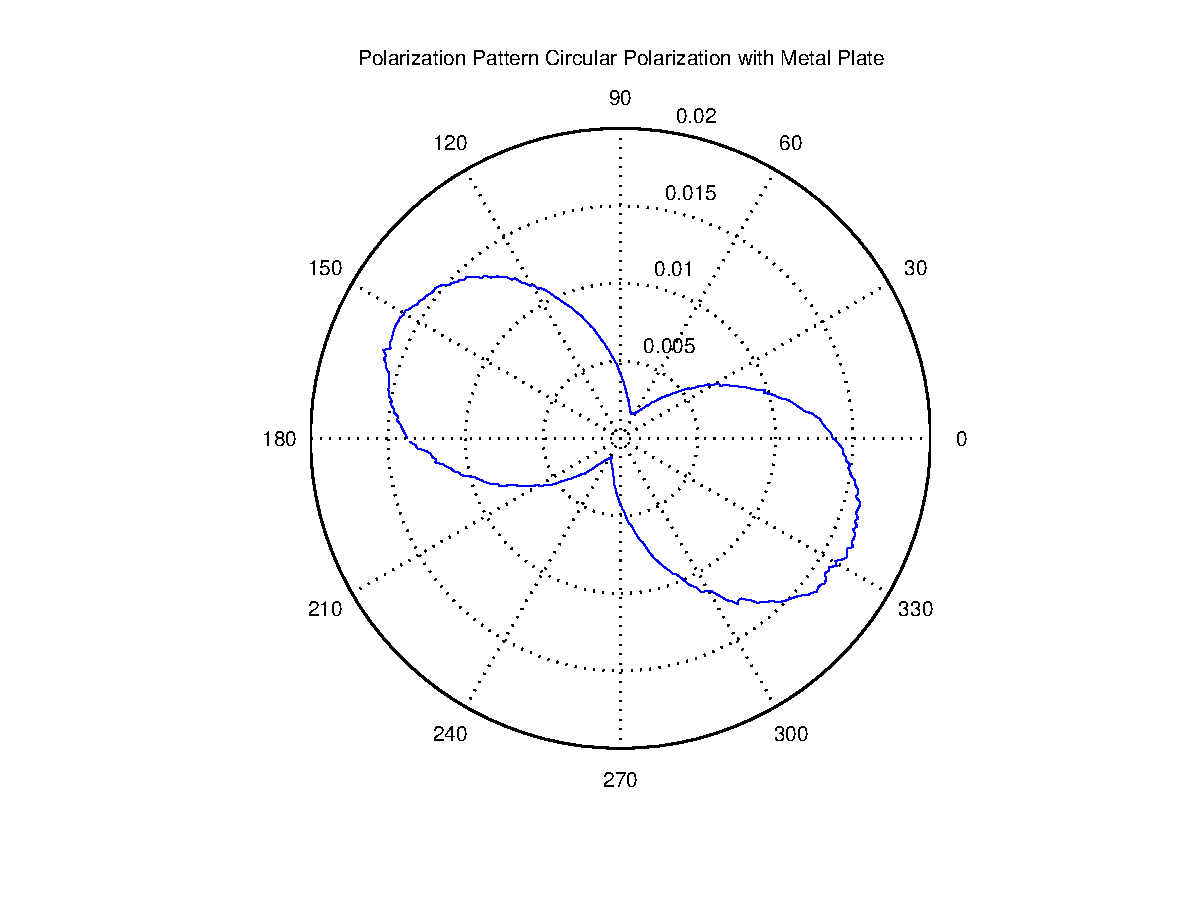
\includegraphics[width=1.2\linewidth]{2_4circ_pol_metal_plate.eps}
  \caption{Circular Polarisation}
  \label{fig:2_4circ}
\end{subfigure}%
\begin{subfigure}{0.5\textwidth}
  \centering
  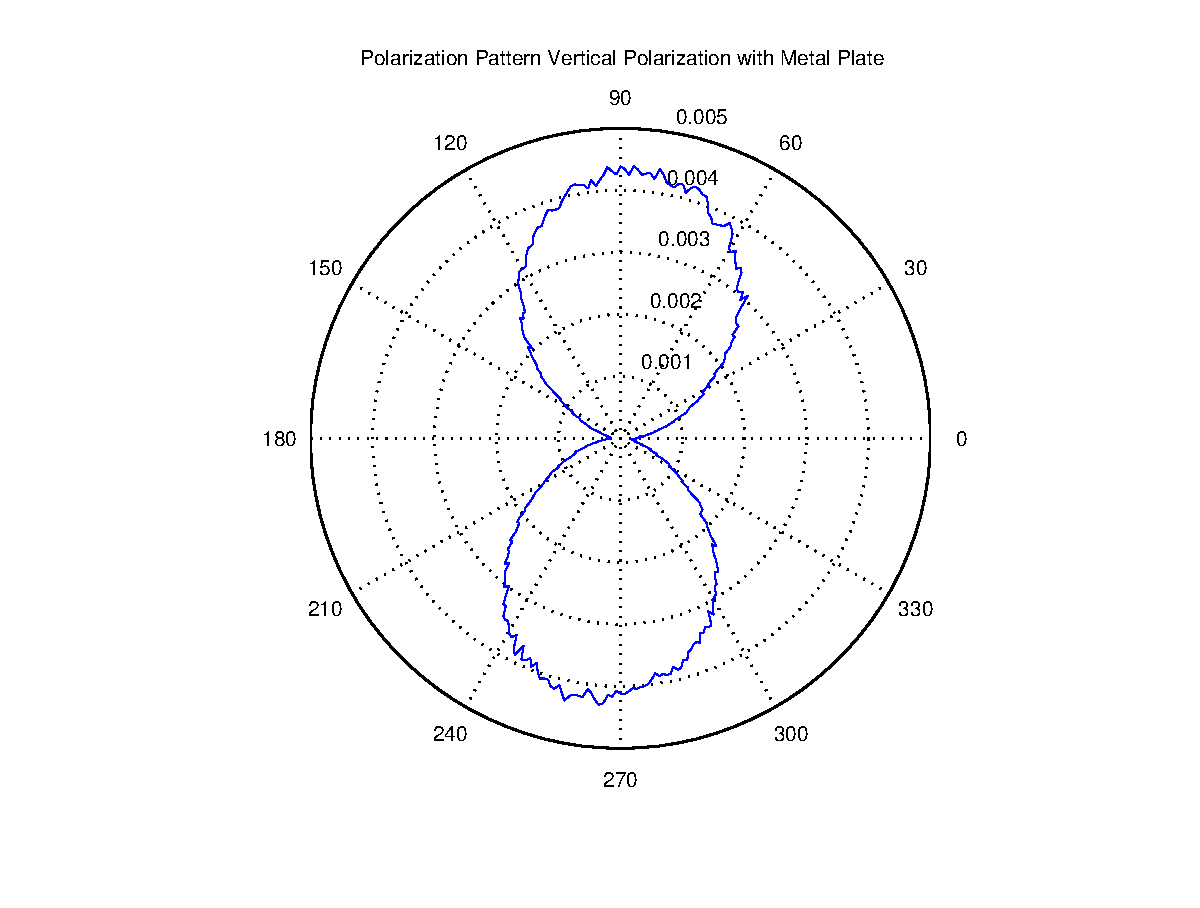
\includegraphics[width=1.2\linewidth]{2_3vert_pol_metal_plate.eps}
  \caption{Vertical Polarisation}
  \label{fig:2_3vert}
\end{subfigure}
\caption{Measured polarisation pattern with the metal plate}
\label{fig:pol_pat_metal_plate}
\end{figure}



\begin{figure}[h]
\begin{center}
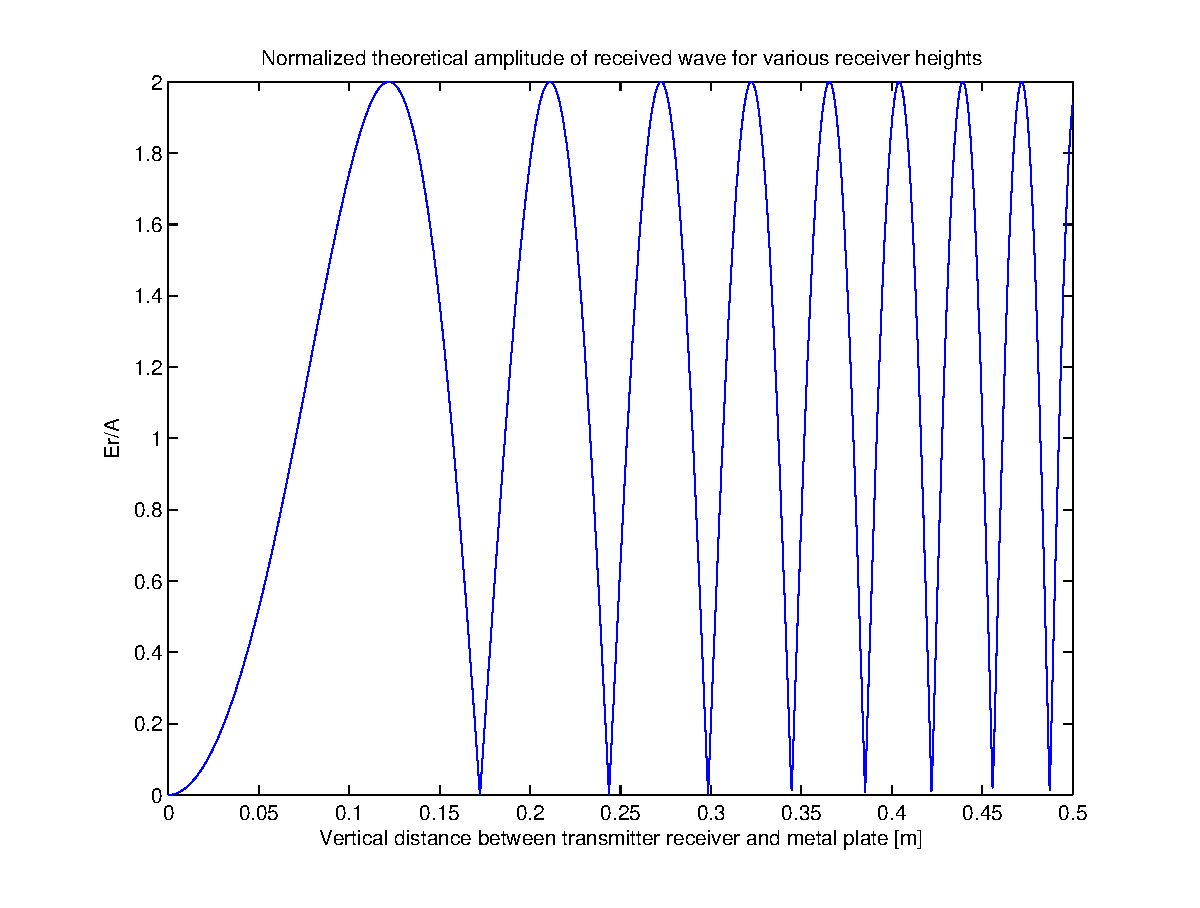
\includegraphics[scale=0.5]{e_zero.eps}
\caption{Theoretical normalized received electric field amplitude}
\label{fig:e_zero}
\end{center}
\end{figure}


%For question 2.5
\begin{figure}[h]
\begin{center}
\includegraphics[scale=0.5]{2_5circ_pol_dielectric_plate}
\caption{Measured polarisation pattern for circular polarisation with the dielectric plate}
\label{fig:2_5circ_diel}
\end{center}
\end{figure}

\section{References}
%[1]  LaTeX tables generated using http://www.tablesgenerator.com/\\
{[1]} H. Mott, \textit{Polarization In Antennas And Radar}. New York: John Wiley and Sons.\\
{[2]} \textit{EE3P11 - EM Practicum, 2015-2016 Q3}, TU Delft, Delft, Netherlands, 2016. \\
{[3]} D. Booms, P. de Vaere, N. du Plessis, J. van Staveren, \textit{EE3P11 Electromagnetics, Practicum Session 1, Transmission Lines}, TU Delft, Delft, Netherlands, 2016.

\end{document}
